\documentclass[aspectratio=169]{beamer}

% Theme and color setup
\usetheme{default}
\usefonttheme{professionalfonts}
\usepackage{amsmath, amssymb}
\usepackage{graphicx}
\usepackage{booktabs}
\usepackage{array}
\usepackage{fontspec}
\usepackage{tikz}
\usetikzlibrary{shapes.geometric, positioning, calc, shadows, fit, arrows.meta}
\usepackage{tcolorbox}
\tcbuselibrary{skins, breakable}
\usepackage{pifont}
\usepackage{tabularx}

% Custom color palette - Blue shades with pastel accents (LIGHTER dark blue)
\definecolor{tmBlue}{RGB}{30,120,180}
\definecolor{tmDarkBlue}{RGB}{45,100,145}
\definecolor{tmLightBlue}{RGB}{100,160,210}
\definecolor{tmLight}{RGB}{230,245,255}
\definecolor{tmLighter}{RGB}{245,250,255}
\definecolor{tmPastelYellow}{RGB}{255,250,230}
\definecolor{tmYellow}{RGB}{255,220,130}
\definecolor{tmPastelPink}{RGB}{255,225,238}
\definecolor{tmPink}{RGB}{255,190,215}
\definecolor{tmGray}{RGB}{60,75,95}
\definecolor{tmGreen}{RGB}{46,139,87}

% Beamer color settings
\setbeamercolor{palette primary}{bg=tmBlue,fg=white}
\setbeamercolor{palette secondary}{bg=tmDarkBlue,fg=white}
\setbeamercolor{palette tertiary}{bg=tmDarkBlue,fg=white}
\setbeamercolor{structure}{fg=tmBlue}
\setbeamercolor{frametitle}{bg=tmBlue,fg=white}
\setbeamercolor{title}{fg=white}
\setbeamercolor{subtitle}{fg=tmLight}
\setbeamercolor{author}{fg=tmLightBlue}
\setbeamercolor{date}{fg=tmLight}
\setbeamercolor{normal text}{fg=tmGray}
\setbeamercolor{block title}{bg=tmBlue,fg=white}
\setbeamercolor{block body}{bg=tmLight,fg=tmGray}
\setbeamercolor{block title alerted}{bg=tmPink,fg=tmDarkBlue}
\setbeamercolor{block body alerted}{bg=tmPastelPink,fg=tmGray}
\setbeamercolor{block title example}{bg=tmYellow,fg=tmDarkBlue}
\setbeamercolor{block body example}{bg=tmPastelYellow,fg=tmGray}
\setbeamercolor{itemize item}{fg=tmBlue}
\setbeamercolor{itemize subitem}{fg=tmLightBlue}
\setbeamercolor{enumerate item}{fg=tmBlue}

% Custom bullet styles
\setbeamertemplate{itemize item}{\color{tmBlue}$\blacktriangleright$}
\setbeamertemplate{itemize subitem}{\color{tmLightBlue}$\bullet$}
\setbeamertemplate{enumerate items}[default]

% Remove navigation symbols, custom footline
\setbeamertemplate{navigation symbols}{}
\setbeamertemplate{footline}{%
  \leavevmode%
  \hbox{%
    \begin{beamercolorbox}[wd=.33\paperwidth,ht=2.5ex,dp=1ex,left]{author in head/foot}%
      \usebeamerfont{author in head/foot}\hspace*{2ex}\textcolor{tmGray}{\insertshortauthor}
    \end{beamercolorbox}%
    \begin{beamercolorbox}[wd=.34\paperwidth,ht=2.5ex,dp=1ex,center]{title in head/foot}%
      \usebeamerfont{title in head/foot}\textcolor{tmBlue}{\insertshorttitle}
    \end{beamercolorbox}%
    \begin{beamercolorbox}[wd=.33\paperwidth,ht=2.5ex,dp=1ex,right]{date in head/foot}%
      \usebeamerfont{date in head/foot}\textcolor{tmGray}{\insertframenumber{} / \inserttotalframenumber}\hspace*{2ex}
    \end{beamercolorbox}}%
  \vskip0pt%
}

% Custom frametitle with decorative bar
\setbeamertemplate{frametitle}{%
  \nointerlineskip%
  \begin{beamercolorbox}[wd=\paperwidth,ht=2.5ex,dp=1ex]{frametitle}
    \hspace*{1.5ex}\insertframetitle
  \end{beamercolorbox}%
  \nointerlineskip%
  
\begin{tikzpicture}[remember picture,overlay]
    \fill[tmYellow] (0,0) rectangle (0.12\paperwidth,2pt);
    \fill[tmPink] (0.12\paperwidth,0) rectangle (0.20\paperwidth,2pt);
  \end{tikzpicture}%
  \vspace{-4pt}%
}

% Font setup
\setmainfont{Latin Modern Roman}

% Custom tcolorbox styles - COMPACT
\newtcolorbox{infobox}[1][]{%
  enhanced,
  colback=tmLight,
  colframe=tmBlue,
  fonttitle=\bfseries\small\color{white},
  boxrule=0.8pt,
  arc=3mm,
  left=4pt, right=4pt, top=2pt, bottom=2pt,
  #1
}

\newtcolorbox{yellowbox}[1][]{%
  enhanced,
  colback=tmPastelYellow,
  colframe=tmYellow,
  fonttitle=\bfseries\small\color{tmDarkBlue},
  boxrule=0.8pt,
  arc=3mm,
  left=4pt, right=4pt, top=2pt, bottom=2pt,
  #1
}

\newtcolorbox{pinkbox}[1][]{%
  enhanced,
  colback=tmPastelPink,
  colframe=tmPink,
  fonttitle=\bfseries\small\color{tmDarkBlue},
  boxrule=0.8pt,
  arc=3mm,
  left=4pt, right=4pt, top=2pt, bottom=2pt,
  #1
}

\newtcolorbox{conceptbox}[2][]{%
  enhanced,
  colback=tmLighter,
  colframe=tmDarkBlue,
  fonttitle=\bfseries\small\color{white},
  colbacktitle=tmDarkBlue,
  coltitle=white,
  title=#2,
  boxrule=1pt,
  arc=3mm,
  left=5pt, right=5pt, top=3pt, bottom=3pt,
  attach boxed title to top left={xshift=4mm,yshift=-2mm},
  boxed title style={arc=2mm, boxrule=0pt},
  #1
}

% Custom commands
\newcommand{\cmark}{\textcolor{tmGreen}{\ding{51}}}
\newcommand{\highlight}[1]{\textcolor{tmBlue}{\textbf{#1}}}

\title[TuniMaqam API]{TuniMaqam API}
\subtitle{Digital Guardian of Tunisian Maqam Heritage}
\author{Roua Smida}
\institute{IT325 Web Services • Tunis Business School}
\date{Academic Year 2025--2026}

\begin{document}

% ============================================================================
% SLIDE 1: Title
% ============================================================================
\begin{frame}[plain]
\begin{tikzpicture}[remember picture,overlay]
  \fill[tmDarkBlue] (current page.south west) rectangle (current page.north east);
  \fill[tmBlue, opacity=0.5] (current page.north east) ++(-2.5,-1.5) circle (3.5cm);
  \fill[tmLightBlue, opacity=0.4] (current page.south west) ++(1.5,1.5) circle (2.5cm);
  \fill[tmPink, opacity=0.25] (current page.north west) ++(3,-3) circle (1.8cm);
  \fill[tmYellow, opacity=0.2] (current page.south east) ++(-4,2.5) circle (2cm);
\end{tikzpicture}

\vspace{1.2cm}
\begin{center}
  {\Huge\bfseries\color{white} TuniMaqam API}\\[0.5cm]
  {\Large\color{tmLight} Digital Guardian of Tunisian Maqam Heritage}\\[1.2cm]
  
  
\begin{tikzpicture}
    \node[draw=tmYellow, line width=1.5pt, rounded corners=6pt, inner sep=10pt, fill=tmDarkBlue, fill opacity=0.6, text opacity=1] {
      \begin{minipage}{0.55\textwidth}
        \centering
        \color{white}
        \textbf{Roua Smida}\\[2pt]
        \small IT325 Web Services • Tunis Business School\\[2pt]
        \small Supervisor: Dr. Montassar Ben Messaoud\\[2pt]
        \small Academic Year 2025--2026
      \end{minipage}
    };
  \end{tikzpicture}
\end{center}
\end{frame}

% ============================================================================
% SLIDE 2: Vision & Mission
% ============================================================================
\begin{frame}{Vision \& Mission}
\vspace{-0.2cm}
\begin{columns}[T]
  \begin{column}{0.47\textwidth}
    \begin{conceptbox}{Our Vision}
      {\small Leverage technology to \highlight{preserve}, \highlight{teach}, and \highlight{promote} Tunisian maqam music (\textit{Tbu'a}) while respecting its cultural authenticity.}
    \end{conceptbox}
    \vspace{0.15cm}
    \begin{yellowbox}[title=Mission Pillars]
      {\small\begin{itemize}\setlength\itemsep{0pt}
        \item[\cmark] \textbf{Preserve} rare maqamet
        \item[\cmark] \textbf{Educate} through engaging learning
        \item[\cmark] \textbf{Connect} generations globally
      \end{itemize}}
    \end{yellowbox}
  \end{column}
  \begin{column}{0.47\textwidth}
    \begin{pinkbox}[title=What is a Maqam?]
      {\small A \textbf{modal framework} defining scales and emotional expressions in Arab music. Tunisia's tradition (\textit{Tab'/Tbu'}) is one of the most sophisticated.}
    \end{pinkbox}
    \vspace{0.15cm}
    \begin{infobox}[title=Production-Ready]
      {\small RESTful API • Containerized • Documented • Secure}
    \end{infobox}
  \end{column}
\end{columns}
\end{frame}

% ============================================================================
% SLIDE 3: Problem Statement
% ============================================================================
\begin{frame}{The Challenge}
\vspace{-0.2cm}
\begin{conceptbox}{Why This Matters}
  {\small Tunisia's maqam tradition has accompanied weddings, celebrations, and spiritual gatherings for centuries—yet this living heritage faces the erosion of time.}
\end{conceptbox}
\vspace{0.15cm}
\begin{columns}[T]
  \begin{column}{0.47\textwidth}
    \begin{pinkbox}[title=Current Challenges]
      {\small\begin{itemize}\setlength\itemsep{1pt}
        \item \textbf{Fragmented Knowledge} — Scattered sources
        \item \textbf{Learning Barriers} — Years of apprenticeship
        \item \textbf{Identification Difficulty} — Rare maqamet
      \end{itemize}}
    \end{pinkbox}
  \end{column}
  \begin{column}{0.47\textwidth}
    \begin{yellowbox}[title=Research Gap]
      {\small No existing system combines:
      \begin{itemize}\setlength\itemsep{0pt}
        \item Structured Tunisian maqam knowledge
        \item Adaptive learning tools
        \item Intelligent analysis \& recommendations
      \end{itemize}
      ...in an accessible API format.}
    \end{yellowbox}
  \end{column}
\end{columns}
\end{frame}

% ============================================================================
% SLIDE 4: Stakeholders
% ============================================================================
\begin{frame}{Stakeholders \& Their Needs}
\begin{center}
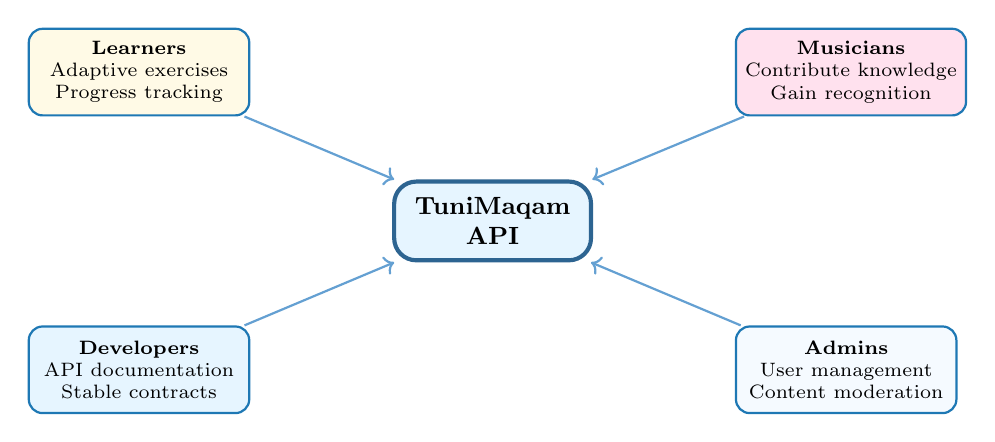
\begin{tikzpicture}[
  box/.style={draw=tmBlue, thick, rounded corners=5pt, minimum width=2.8cm, minimum height=1.1cm, align=center, font=\scriptsize},
  arrow/.style={->, thick, tmLightBlue}
]
  \node[draw=tmDarkBlue, line width=1.5pt, rounded corners=8pt, minimum width=2.5cm, minimum height=1cm, fill=tmLight, align=center, font=\small\bfseries] (api) {TuniMaqam\\API};
  
  \node[box, fill=tmPastelYellow, above left=0.8cm and 1.8cm of api] (learner) {\textbf{Learners}\\Adaptive exercises\\Progress tracking};
  \node[box, fill=tmPastelPink, above right=0.8cm and 1.8cm of api] (expert) {\textbf{Musicians}\\Contribute knowledge\\Gain recognition};
  \node[box, fill=tmLight, below left=0.8cm and 1.8cm of api] (dev) {\textbf{Developers}\\API documentation\\Stable contracts};
  \node[box, fill=tmLighter, below right=0.8cm and 1.8cm of api] (admin) {\textbf{Admins}\\User management\\Content moderation};
  
  \draw[arrow] (learner) -- (api);
  \draw[arrow] (expert) -- (api);
  \draw[arrow] (dev) -- (api);
  \draw[arrow] (admin) -- (api);
\end{tikzpicture}
\end{center}
\end{frame}

% ============================================================================
% SLIDE 5: Architecture Overview
% ============================================================================
\begin{frame}{System Architecture}
\vspace{-0.2cm}
\begin{columns}[T]
  \begin{column}{0.52\textwidth}
    \begin{center}
    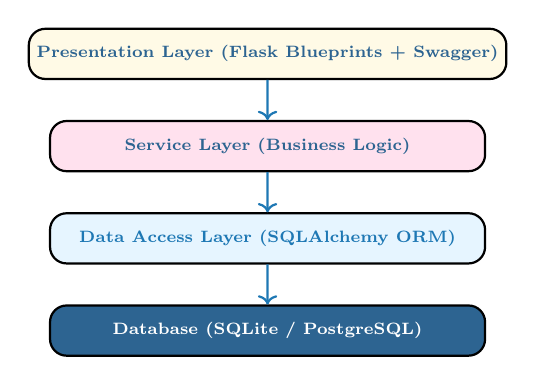
\begin{tikzpicture}[node distance=0.6cm, scale=0.85, transform shape]
      \node[draw, thick, rounded corners=6pt, minimum width=6.5cm, minimum height=0.75cm, fill=tmPastelYellow, text=tmDarkBlue, font=\bfseries\scriptsize] (pres) {Presentation Layer (Flask Blueprints + Swagger)};
      \node[draw, thick, rounded corners=6pt, below=of pres, minimum width=6.5cm, minimum height=0.75cm, fill=tmPastelPink, text=tmDarkBlue, font=\bfseries\scriptsize] (svc) {Service Layer (Business Logic)};
      \node[draw, thick, rounded corners=6pt, below=of svc, minimum width=6.5cm, minimum height=0.75cm, fill=tmLight, text=tmBlue, font=\bfseries\scriptsize] (data) {Data Access Layer (SQLAlchemy ORM)};
      \node[draw, thick, rounded corners=6pt, below=of data, minimum width=6.5cm, minimum height=0.75cm, fill=tmDarkBlue, text=white, font=\bfseries\scriptsize] (db) {Database (SQLite / PostgreSQL)};
      
      \draw[->, thick, tmBlue] (pres) -- (svc);
      \draw[->, thick, tmBlue] (svc) -- (data);
      \draw[->, thick, tmBlue] (data) -- (db);
    \end{tikzpicture}
    \end{center}
  \end{column}
  \begin{column}{0.44\textwidth}
    \begin{infobox}[title=Tech Stack]
      {\small\begin{itemize}\setlength\itemsep{0pt}
        \item \textbf{Flask 3.x} — Web Framework
        \item \textbf{SQLAlchemy} — ORM
        \item \textbf{Marshmallow} — Validation
        \item \textbf{PyJWT + Authlib} — Auth
        \item \textbf{Flasgger} — API Docs
        \item \textbf{Docker} — Deployment
      \end{itemize}}
    \end{infobox}
  \end{column}
\end{columns}
\end{frame}

% ============================================================================
% SLIDE 6: Data Model
% ============================================================================
\begin{frame}{Data Model}
\vspace{-0.2cm}
\begin{columns}[T]
  \begin{column}{0.42\textwidth}
    \begin{center}
    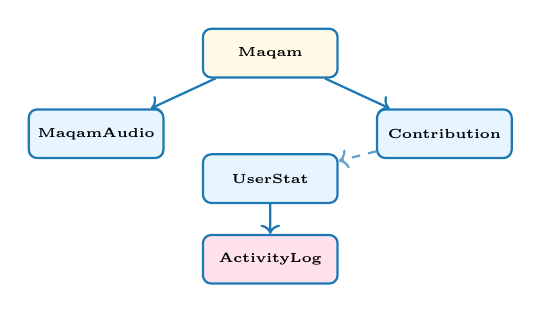
\begin{tikzpicture}[
      entity/.style={draw=tmBlue, thick, rounded corners=3pt, minimum width=1.8cm, minimum height=0.65cm, fill=tmLight, font=\tiny\bfseries},
      node distance=0.4cm and 0.5cm,
      scale=0.95, transform shape
    ]
      \node[entity, fill=tmPastelYellow] (maqam) {Maqam};
      \node[entity, below left=of maqam] (audio) {MaqamAudio};
      \node[entity, below right=of maqam] (contrib) {Contribution};
      \node[entity, below=1cm of maqam] (user) {UserStat};
      \node[entity, below=of user, fill=tmPastelPink] (log) {ActivityLog};
      
      \draw[->, thick, tmBlue] (maqam) -- (audio);
      \draw[->, thick, tmBlue] (maqam) -- (contrib);
      \draw[->, thick, tmBlue] (user) -- (log);
      \draw[->, thick, tmLightBlue, dashed] (contrib) -- (user);
    \end{tikzpicture}
    \end{center}
  \end{column}
  \begin{column}{0.54\textwidth}
    \begin{yellowbox}[title=Key Features]
      {\small\begin{itemize}\setlength\itemsep{0pt}
        \item \textbf{Bilingual} names (Arabic/English)
        \item \textbf{Ajnas} stored as JSON
        \item \textbf{Emotion weights} for mood queries
        \item \textbf{Contribution workflow} with audit
      \end{itemize}}
    \end{yellowbox}
    \vspace{0.1cm}
    \begin{pinkbox}[title=Maqam Attributes]
      {\scriptsize Name • Region • Emotion • Difficulty • Rarity • Usage • Related}
    \end{pinkbox}
  \end{column}
\end{columns}
\end{frame}

% ============================================================================
% SLIDE 7: Four Core Services
% ============================================================================
\begin{frame}{Four Core Services}
\begin{center}
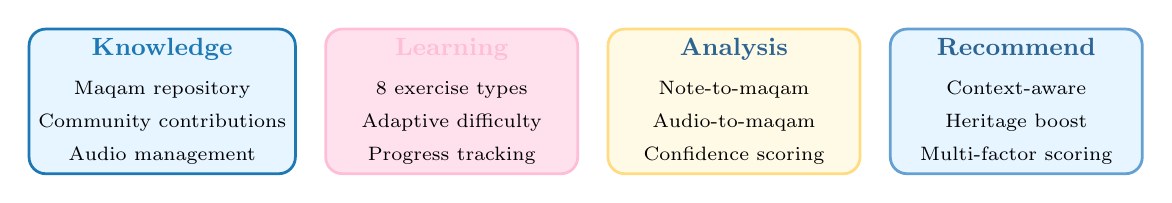
\begin{tikzpicture}[node distance=0.35cm]
  \node[draw=tmBlue, line width=1pt, rounded corners=6pt, minimum width=3.2cm, minimum height=1.8cm, align=center, fill=tmLight] (know) {
    \textbf{\small\color{tmBlue}Knowledge}\\[2pt]
    {\scriptsize Maqam repository}\\
    {\scriptsize Community contributions}\\
    {\scriptsize Audio management}
  };
  \node[draw=tmPink, line width=1pt, rounded corners=6pt, minimum width=3.2cm, minimum height=1.8cm, align=center, fill=tmPastelPink, right=of know] (learn) {
    \textbf{\small\color{tmPink}Learning}\\[2pt]
    {\scriptsize 8 exercise types}\\
    {\scriptsize Adaptive difficulty}\\
    {\scriptsize Progress tracking}
  };
  \node[draw=tmYellow, line width=1pt, rounded corners=6pt, minimum width=3.2cm, minimum height=1.8cm, align=center, fill=tmPastelYellow, right=of learn] (anal) {
    \textbf{\small\color{tmDarkBlue}Analysis}\\[2pt]
    {\scriptsize Note-to-maqam}\\
    {\scriptsize Audio-to-maqam}\\
    {\scriptsize Confidence scoring}
  };
  \node[draw=tmLightBlue, line width=1pt, rounded corners=6pt, minimum width=3.2cm, minimum height=1.8cm, align=center, fill=tmLight, right=of anal] (rec) {
    \textbf{\small\color{tmDarkBlue}Recommend}\\[2pt]
    {\scriptsize Context-aware}\\
    {\scriptsize Heritage boost}\\
    {\scriptsize Multi-factor scoring}
  };
\end{tikzpicture}
\end{center}
\vspace{0.15cm}
\begin{conceptbox}{Integrated Platform}
  {\small All services work together: Analysis identifies maqamet $\rightarrow$ Learning creates quizzes $\rightarrow$ Recommendations suggest next steps $\rightarrow$ Knowledge preserves contributions.}
\end{conceptbox}
\end{frame}

% ============================================================================
% SLIDE 8: Knowledge Service
% ============================================================================
\begin{frame}{Knowledge Service}
\vspace{-0.2cm}
\begin{columns}[T]
  \begin{column}{0.47\textwidth}
    \begin{infobox}[title=API Endpoints]
      {\scriptsize\begin{tabular}{ll}
        \textbf{GET} & \texttt{/knowledge/maqam}\\
        \textbf{GET} & \texttt{/maqam/\{id\}}\\
        \textbf{GET} & \texttt{/maqam/by-name/\{n\}}\\
        \textbf{POST} & \texttt{/maqam} (admin)\\
      \end{tabular}}
    \end{infobox}
    \vspace{0.1cm}
    \begin{pinkbox}[title=Audio Management]
      {\small\begin{itemize}\setlength\itemsep{0pt}
        \item Upload MP3, WAV, OGG
        \item Validation \& secure storage
      \end{itemize}}
    \end{pinkbox}
  \end{column}
  \begin{column}{0.47\textwidth}
    \begin{yellowbox}[title=Contribution Workflow]
      {\small\begin{enumerate}\setlength\itemsep{0pt}
        \item User submits contribution
        \item Status: \texttt{pending}
        \item Expert/Admin reviews
        \item \texttt{accepted} or \texttt{rejected}
      \end{enumerate}}
    \end{yellowbox}
    \vspace{0.1cm}
    \begin{block}{\small Contribution Types}
      {\scriptsize\texttt{new\_maqam} • \texttt{correction} • \texttt{addition} • \texttt{audio}}
    \end{block}
  \end{column}
\end{columns}
\end{frame}

% ============================================================================
% SLIDE 9: Learning Service
% ============================================================================
\begin{frame}{Learning Service}
\vspace{-0.2cm}
\begin{columns}[T]
  \begin{column}{0.50\textwidth}
    \begin{conceptbox}{8 Exercise Types}
      \begin{center}
      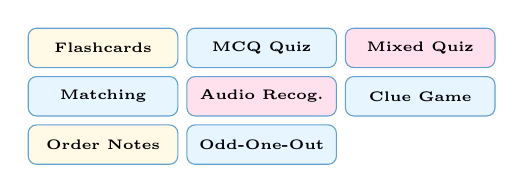
\begin{tikzpicture}[
        ex/.style={draw=tmLightBlue, rounded corners=3pt, minimum width=1.9cm, minimum height=0.5cm, font=\tiny\bfseries, fill=tmLight},
        node distance=0.1cm
      ]
        \node[ex, fill=tmPastelYellow] (fc) {Flashcards};
        \node[ex, right=of fc] (mcq) {MCQ Quiz};
        \node[ex, right=of mcq, fill=tmPastelPink] (mix) {Mixed Quiz};
        \node[ex, below=of fc] (match) {Matching};
        \node[ex, right=of match, fill=tmPastelPink] (audio) {Audio Recog.};
        \node[ex, right=of audio] (clue) {Clue Game};
        \node[ex, below=of match, fill=tmPastelYellow] (order) {Order Notes};
        \node[ex, right=of order] (odd) {Odd-One-Out};
      \end{tikzpicture}
      \end{center}
    \end{conceptbox}
    \vspace{0.1cm}
    \begin{pinkbox}[title=Pedagogy]
      {\scriptsize Active Recall • Spaced Repetition • Immediate Feedback}
    \end{pinkbox}
  \end{column}
  \begin{column}{0.46\textwidth}
    \begin{yellowbox}[title=Adaptive Difficulty]
      {\small Learner level computed dynamically:\\[2pt]
      \textbf{Advanced:} score $\geq$ 75\% \& 10+ activities\\
      \textbf{Intermediate:} score $\geq$ 50\% or 5+\\
      \textbf{Beginner:} otherwise}
    \end{yellowbox}
    \vspace{0.1cm}
    \begin{infobox}[title=Gamification]
      {\small Points • Streaks • Leaderboard • Progress}
    \end{infobox}
  \end{column}
\end{columns}
\end{frame}

% ============================================================================
% SLIDE 10: Analysis Engine (MERGED)
% ============================================================================
\begin{frame}{Analysis Engine}
\vspace{-0.2cm}
\begin{columns}[T]
  \begin{column}{0.48\textwidth}
    \begin{conceptbox}{First Jins Focus}
      {\small The \textbf{first jins} contains the tonic and characteristic intervals—the ``DNA'' of the maqam.}
    \end{conceptbox}
    \vspace{0.1cm}
    \begin{yellowbox}[title=Confidence Formula]
      {\small $\text{Conf} = \text{Base} \times \text{Mult}$\\[2pt]
      $\text{Base} = 0.7 \cdot \frac{|C|}{|I|} + 0.3 \cdot \frac{|C|}{|M|}$\\[2pt]
      {\scriptsize $I$ = input, $M$ = maqam notes, $C$ = common}}
    \end{yellowbox}
  \end{column}
  \begin{column}{0.48\textwidth}
    \begin{pinkbox}[title=Match Multiplier]
      \begin{center}
      {\scriptsize\begin{tabular}{cc}
        \textbf{Matches} & \textbf{Mult}\\
        \hline
        1 & 0.50\\
        2 & 0.70\\
        3--4 & 0.85--0.95\\
        5+ & 1.00\\
      \end{tabular}}
      \end{center}
    \end{pinkbox}
    \vspace{0.1cm}
    \begin{infobox}[title=Audio Pipeline]
      {\scriptsize Upload $\rightarrow$ AssemblyAI $\rightarrow$ Extract Notes $\rightarrow$ Analyze $\rightarrow$ Return Candidates}
    \end{infobox}
  \end{column}
\end{columns}
\end{frame}

% ============================================================================
% SLIDE 11: Recommendation Engine
% ============================================================================
\begin{frame}{Recommendation Engine}
\vspace{-0.2cm}
\begin{columns}[T]
  \begin{column}{0.48\textwidth}
    \begin{conceptbox}{Multi-Factor Scoring}
      {\small $S_m = \sum_i w_i \cdot f_i(m)$\\[2pt]
      Score for maqam $m$ based on weighted factors.}
    \end{conceptbox}
    \vspace{0.1cm}
    \begin{infobox}[title=Scoring Factors]
      {\scriptsize\begin{tabular}{lc}
        \textbf{Factor} & \textbf{Max}\\
        \hline
        Mood alignment & +1.0\\
        Event match & +0.25\\
        Region match & +0.20\\
        Heritage boost & +0.20\\
      \end{tabular}}
    \end{infobox}
  \end{column}
  \begin{column}{0.48\textwidth}
    \begin{pinkbox}[title=Heritage Preservation]
      {\small Rare and endangered maqamet receive a \textbf{+20\%} boost for cultural preservation.}
    \end{pinkbox}
    \vspace{0.1cm}
    \begin{yellowbox}[title=Example Request]
      {\scriptsize\texttt{\{"mood": "joy", "event": "wedding", "region": "tunis"\}}}\\[2pt]
      {\small Returns ranked suggestions with rationale.}
    \end{yellowbox}
  \end{column}
\end{columns}
\end{frame}

% ============================================================================
% SLIDE 12: Security & Authentication
% ============================================================================
\begin{frame}{Security \& Authentication}
\vspace{-0.2cm}
\begin{columns}[T]
  \begin{column}{0.46\textwidth}
    \begin{conceptbox}{Role-Based Access Control}
      \begin{center}
      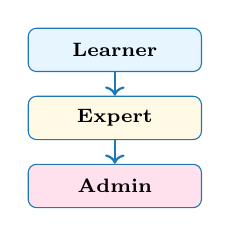
\begin{tikzpicture}[
        role/.style={draw=tmBlue, rounded corners=3pt, minimum width=2.2cm, minimum height=0.55cm, font=\scriptsize\bfseries},
        node distance=0.3cm
      ]
        \node[role, fill=tmLight] (learner) {Learner};
        \node[role, fill=tmPastelYellow, below=of learner] (expert) {Expert};
        \node[role, fill=tmPastelPink, below=of expert] (admin) {Admin};
        
        \draw[->, thick, tmBlue] (learner) -- (expert);
        \draw[->, thick, tmBlue] (expert) -- (admin);
      \end{tikzpicture}
      \end{center}
      {\small\centering Hierarchical permissions}
    \end{conceptbox}
  \end{column}
  \begin{column}{0.50\textwidth}
    \begin{yellowbox}[title=JWT Authentication]
      {\small\begin{itemize}\setlength\itemsep{0pt}
        \item Industry-standard tokens
        \item Role embedded in claims
        \item Configurable expiration
      \end{itemize}}
    \end{yellowbox}
    \vspace{0.1cm}
    \begin{pinkbox}[title=Security Features]
      {\small\begin{itemize}\setlength\itemsep{0pt}
        \item[\cmark] Google OAuth 2.0
        \item[\cmark] Rate limiting (Flask-Limiter)
        \item[\cmark] Input validation (Marshmallow)
        \item[\cmark] CORS \& RESTful errors
      \end{itemize}}
    \end{pinkbox}
  \end{column}
\end{columns}
\end{frame}

% ============================================================================
% SLIDE 13: API Surface
% ============================================================================
\begin{frame}{API Surface}
\begin{center}
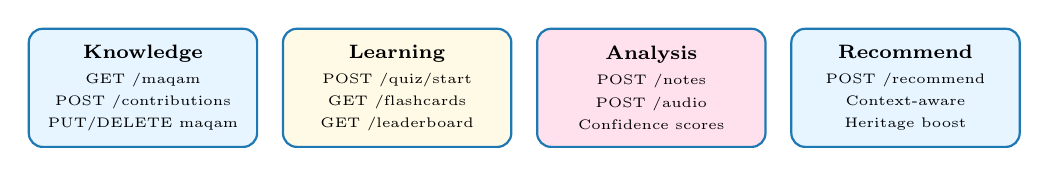
\begin{tikzpicture}[
  api/.style={draw=tmBlue, thick, rounded corners=5pt, minimum width=2.9cm, minimum height=1.5cm, align=center, font=\scriptsize},
  node distance=0.3cm
]
  \node[api, fill=tmLight] (know) {\textbf{Knowledge}\\[1pt]{\tiny GET /maqam}\\{\tiny POST /contributions}\\{\tiny PUT/DELETE maqam}};
  \node[api, fill=tmPastelYellow, right=of know] (learn) {\textbf{Learning}\\[1pt]{\tiny POST /quiz/start}\\{\tiny GET /flashcards}\\{\tiny GET /leaderboard}};
  \node[api, fill=tmPastelPink, right=of learn] (anal) {\textbf{Analysis}\\[1pt]{\tiny POST /notes}\\{\tiny POST /audio}\\{\tiny Confidence scores}};
  \node[api, fill=tmLight, right=of anal] (rec) {\textbf{Recommend}\\[1pt]{\tiny POST /recommend}\\{\tiny Context-aware}\\{\tiny Heritage boost}};
\end{tikzpicture}
\end{center}
\vspace{0.15cm}
\begin{columns}[T]
  \begin{column}{0.47\textwidth}
    \begin{infobox}[title=Interactive Docs]
      {\small Swagger UI at \texttt{/apidocs} — auto-generated}
    \end{infobox}
  \end{column}
  \begin{column}{0.47\textwidth}
    \begin{yellowbox}[title=RESTful Design]
      {\small Standard HTTP verbs • JSON • Consistent errors}
    \end{yellowbox}
  \end{column}
\end{columns}
\end{frame}

% ============================================================================
% SLIDE 14: Testing & Deployment
% ============================================================================
\begin{frame}{Testing \& Deployment}
\vspace{-0.2cm}
\begin{columns}[T]
  \begin{column}{0.47\textwidth}
    \begin{conceptbox}{Test Suite}
      {\small\textbf{Pytest} covers all core services:
      \begin{itemize}\setlength\itemsep{0pt}
        \item \texttt{test\_auth.py}
        \item \texttt{test\_learning.py}
        \item \texttt{test\_analysis.py}
        \item \texttt{test\_recommendations.py}
      \end{itemize}}
    \end{conceptbox}
    \vspace{0.1cm}
    \begin{infobox}[title=Code Quality]
      {\small PEP 8 • Modular blueprints • Separation of concerns}
    \end{infobox}
  \end{column}
  \begin{column}{0.47\textwidth}
    \begin{yellowbox}[title=Containerization]
      {\small\begin{itemize}\setlength\itemsep{0pt}
        \item[\cmark] Dockerfile + Docker Compose
        \item[\cmark] Render.yaml for deployment
        \item[\cmark] SQLite (dev) / PostgreSQL (prod)
        \item[\cmark] Environment variables for secrets
      \end{itemize}}
    \end{yellowbox}
    \vspace{0.1cm}
    \begin{pinkbox}[title=Production Ready]
      {\small Gunicorn • Health checks • Logging}
    \end{pinkbox}
  \end{column}
\end{columns}
\end{frame}

% ============================================================================
% SLIDE 15: Impact & Future Work
% ============================================================================
\begin{frame}{Impact \& Future Work}
\vspace{-0.2cm}
\begin{columns}[T]
  \begin{column}{0.47\textwidth}
    \begin{conceptbox}{Cultural Impact}
      {\small TuniMaqam \textbf{democratizes access} to maqam knowledge—bridging heritage and technology for future generations.}
    \end{conceptbox}
    \vspace{0.1cm}
    \begin{pinkbox}[title=Achievements]
      {\small\begin{itemize}\setlength\itemsep{0pt}
        \item[\cmark] Complete REST API platform
        \item[\cmark] 4 integrated services
        \item[\cmark] Production-ready deployment
        \item[\cmark] Comprehensive documentation
      \end{itemize}}
    \end{pinkbox}
  \end{column}
  \begin{column}{0.47\textwidth}
    \begin{yellowbox}[title=Future Roadmap]
      {\small\begin{itemize}\setlength\itemsep{0pt}
        \item \textbf{Audio Corpus} — Expand recordings
        \item \textbf{ML Models} — Deep learning on audio
        \item \textbf{Mobile Apps} — iOS/Android clients
        \item \textbf{Broader Scope} — Pan-Arab maqamat
      \end{itemize}}
    \end{yellowbox}
    \vspace{0.1cm}
    \begin{infobox}[title=Vision]
      {\small\textbf{Algorithmic cultural preservation at scale.}}
    \end{infobox}
  \end{column}
\end{columns}
\end{frame}

% ============================================================================
% SLIDE 16: Thank You
% ============================================================================
\begin{frame}[plain]
\begin{tikzpicture}[remember picture,overlay]
  \fill[tmDarkBlue] (current page.south west) rectangle (current page.north east);
  \fill[tmBlue, opacity=0.5] (current page.north west) ++(3,-2.5) circle (3cm);
  \fill[tmPink, opacity=0.3] (current page.south east) ++(-3,2.5) circle (3.5cm);
  \fill[tmYellow, opacity=0.25] (current page.center) ++(4,-0.5) circle (1.8cm);
  \fill[tmLightBlue, opacity=0.35] (current page.south west) ++(2,1.5) circle (2cm);
\end{tikzpicture}

\vspace{1.5cm}
\begin{center}
  {\Huge\bfseries\color{white} Thank You!}\\[0.8cm]
  
  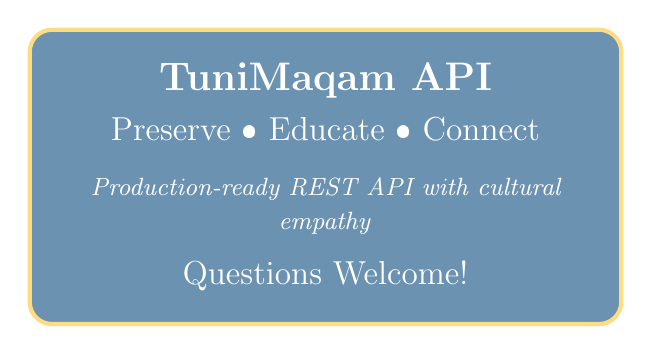
\begin{tikzpicture}
    \node[draw=tmYellow, line width=1.5pt, rounded corners=8pt, inner sep=12pt, fill=tmDarkBlue, fill opacity=0.7, text opacity=1] {
      \begin{minipage}{0.55\textwidth}
        \centering
        \color{white}
        {\Large\bfseries TuniMaqam API}\\[6pt]
        {\large Preserve • Educate • Connect}\\[8pt]
        \textit{\small Production-ready REST API with cultural empathy}\\[8pt]
        {\large Questions Welcome!}
      \end{minipage}
    };
  \end{tikzpicture}
\end{center}
\end{frame}

\end{document}